
\title{\vspace{-5cm} BER Exercise Telecommunication Systems}
\author{
By : Martyn van Dijke \\ Student number : 0887668
}
\date{\today}

\documentclass[12pt]{article}
\usepackage{amsmath}
\usepackage{graphicx}
\usepackage{epstopdf}
\usepackage{floatrow}
\usepackage{minted}
\usepackage{mdframed}
\usepackage{caption}
%\usepackage[newfloat]{minted}

\begin{document}

\maketitle
\noindent Appendix A lists the Mathlab code for the (sub) assignments.\\




  \setlength{\parskip}{0pt}
1 The Matlab implementation of the 7 and 15 bit Hamming encoder can be found in Listings \ref{lst:enc} \\


2 The Matlab implementation of the 7 and 15 bit Hamming decoder can be found in Listings \ref{lst:dec}\\



3 The PRBS signal is generated by the LTE Systems Toolbox, the code for the PRBS sequence can be seen in the PRBS section of the main program which can be found in Listings \ref{lst:main}\\

%throughout the rest of this report these PRBS sequence's are referenced by seq1, seq2. The code for the PRBS sequence can be seen in Listings \ref{lst:main}


4 The Matlab implementation of (white Gaussian) noise with varying  signal to noise amplitude can be seen in Listings \ref{lst:noise} .\\
A plot of BER as a function of the signal to noise ratio can be seen in Figure \ref{fig:seq3} and  Figure \ref{fig:seq2} respectively.
Where Figure \ref{fig:seq2} is made with a PRBS length of $2^{11}-1 $ and Figure \ref{fig:seq3} with a PRBS length of $2^{7}-1 $ \\


5 The improved BER can be seen in Figure \ref{fig:seq3} and in Figure \ref{fig:seq2}.\\ %the difference between Hamming encoded bit stream's and the reference value are
Using these figures the coding gain can be approximated, using this approximation it is clearly notable  that until a SNR value of 5dB the BER of the Hamming code is $ \approx 0.1 - 0.5 $ worse then the reference signal.\\
This is a sensible result of executing the Hamming code at low SNR values, since there are a lot of error's in the signal caused by the high influence of the noise factor. In fact there are more then one bit errors  in the signal per 7 or 15 bit transmission, therefore the Hamming code will try to correct the wrong bits.
This is because Hamming code is a one bit correction and a two bit detection algorithm. \\
After the SNR = 5 dB point the coding gain is $ \approx 2-3 $ dB better then the reference signal.
In this region the amount of errors is lower or equal to 1 error per 7 or 15 bit transmission and thus the Hamming code can correctly detect and repair wrongly received bits.\\

\clearpage

6 As can be seen in Figure\ref{fig:seq3} and in Figure \ref{fig:seq2} the 15 bit transmission system has a slightly higher overall error rate, which is coherent with the theory of Hamming code since on average the 15 bit transmission will have more errors in the received signal as compared to the 7 bit transmission and thus resulting in correcting wrongly received bits.\\
This is the reason why there is there is no coding gain improvement between the 7 bit and 15 bit transmission, there is actually a small coding gain deterioration between the 15 bit and the 7 bit Hamming encoded transmission.
%substantial for a signal to noise ratio of about $15 dB$ after this point the difference in bit errors between coded Hamming and the reference decline fast.\\
%Resulting in a lower coding gain, the coding gain as a function per signal to noise ratio can be seen in Figure \ref{fig:gain}.\\
%Where it is clearly visible that the coding gain converges to 0 for higher signal to noise ratio's
\begin{figure}[H]
    \centering
    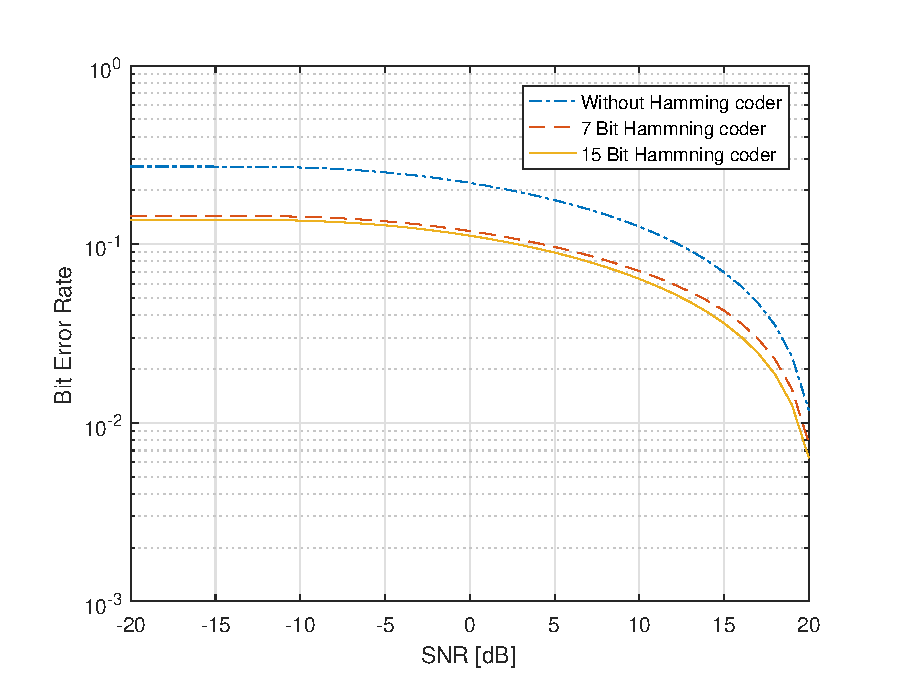
\includegraphics[height=12cm]{PlotSeq3.eps}
    \caption{Bit Error Rate with a PRBS lengths of $2^{7} -1$}
    \label{fig:seq3}
\end{figure}

\begin{figure}[H]
    \centering
    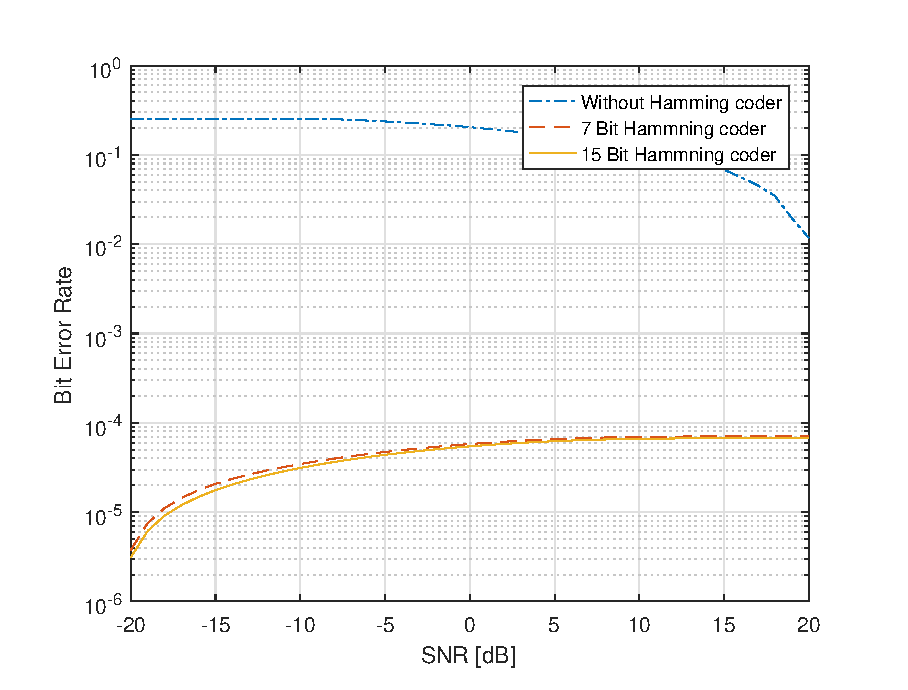
\includegraphics[height=12cm]{PlotSeq2.eps}
    \caption{Bit Error Rate with a PRBS lengths of $2^{11}-1 $}
    \label{fig:seq2}
\end{figure}



%\begin{figure}[H]
%    \centering
%    \includegraphics[height=8cm]{Gain.eps}
%    \caption{Coding Gain}
%    \label{fig:gain}
%\end{figure}


%does have a better overall performance but the margin of improvement as compared to the 7 bit transmission system are low.

\clearpage
\section{Appendix A}
\inputminted{matlab}{DataEncoder.m}
\captionof{listing}{Hamming Encoder \label{lst:enc}}

\inputminted{matlab}{DataDecoder.m}
\captionof{listing}{Hamming Decoder \label{lst:dec}}

\inputminted{matlab}{Decision.m}
\captionof{listing}{Decision Code \label{lst:des}}

\inputminted{matlab}{Noise.m}
\captionof{listing}{Noise Code \label{lst:noise}}


\inputminted{matlab}{main.m}
\captionof{listing}{Main Code \label{lst:main}}









\end{document} 